% article example for classicthesis.sty
\documentclass[10pt,a4paper]{article} % KOMA-Script article scrartcl
\usepackage{lipsum}     %lorem ipsum text
\usepackage{titlesec}   %Section settings
\usepackage{titling}    %Title settings
\usepackage[margin=10em]{geometry}  %Adjusting margins
\usepackage{setspace}
\usepackage{listings}
\usepackage{amsmath}    %Display equations options
\usepackage{amssymb}    %More symbols
\usepackage{xcolor}     %Color settings
\usepackage{pagecolor}
\usepackage{mdframed}
\usepackage[spanish]{babel}
\usepackage[utf8]{inputenc}
\usepackage{longtable}
\usepackage{multicol}
\usepackage{graphicx}
\graphicspath{ {./Images/} }
\setlength{\columnsep}{1cm}

% ====| color de la pagina y del fondo |==== %
\pagecolor{black}
\color{white}



\begin{document}
    %========================{TITLE}====================%
    \title{\rmfamily\normalfont\spacedallcaps{ Vectores Aleatorios y Matrices Aleatorias }}
    \author{\spacedlowsmallcaps{Rodrigo Castillo}}
    \date{\today} 
    
    \maketitle
     

     % ====| Loguito |==== %
    
\includegraphics[width=0.1\linewidth]{negro_cara.png}
    %=======================NOTES GOES HERE===================%
    \section{Ejercicio de la clase pasada}
        sea 
        \begin{equation}
            A ^{ \frac{1}{2}}  = \sum_{i=1}^{m} \sqrt{\lambda } e_i e_i ^{'}  = PA ^{ \frac{1}{2}} P ^{'}  donde PP ^{'}  = P ^{'}P = 1 
        \end{equation}
        demuestre las cuatro propiedades de la raiz cuadrada de una matriz

    \section{Matrices aleatorias}
        la idea de las matrices aleatorias es generar unas matrices de
        distribucion normal y se pone la esperanza.
        \subsection{Valor esperado de una matriz aleatoria}
            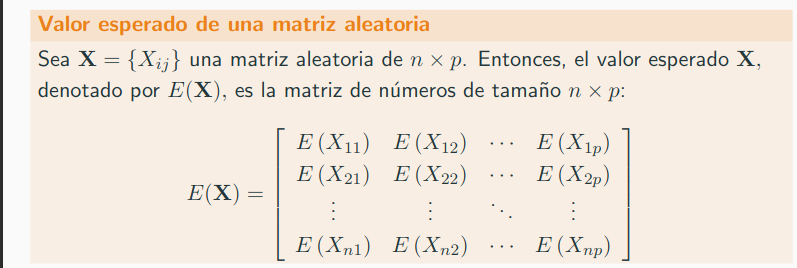
\includegraphics[width=0.8\linewidth]{valoresperadom.png}
        \subsection{Valor esperado sumas de matrices aleatorias}
            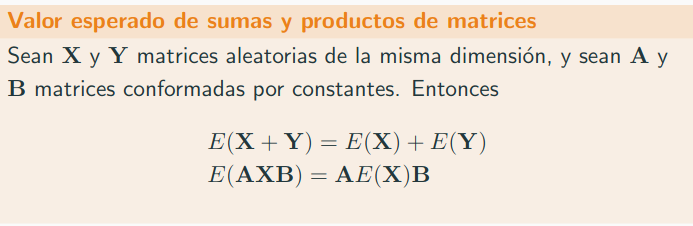
\includegraphics[width=0.8\linewidth]{valorsumasproductosm.png}
        \subsection{Vectores media y matrices de covarianza}
            \subsubsection{vector de medias}
                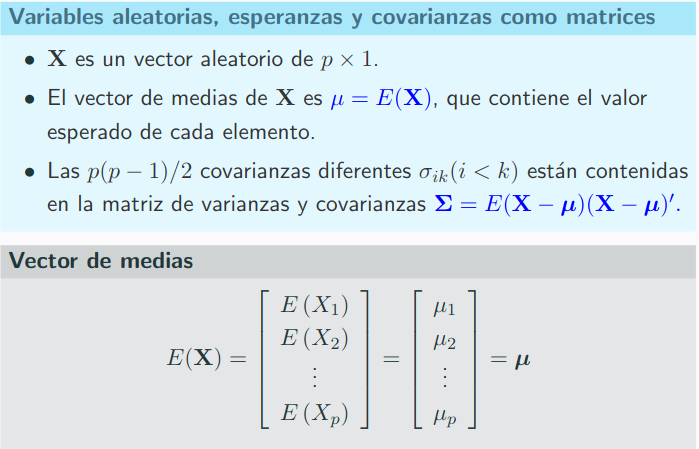
\includegraphics[width=0.8\linewidth]{vectormedias.png} 
             \subsubsection{matriz de covarianzas}
                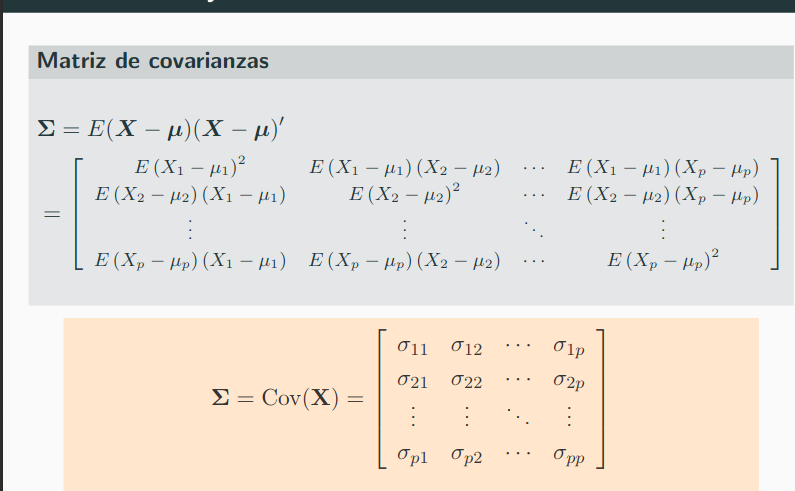
\includegraphics[width=0.8\linewidth]{matrizcovarianzas.png}
         \subsection{coeficiente correlacional}
             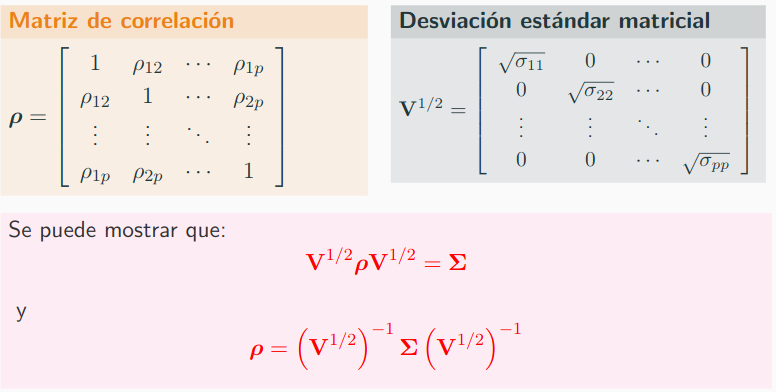
\includegraphics[width=0.8\linewidth]{matrizcorrelacion.png}
            
            \section{Preguntas}
                preguntar el finals sobre la parte de las combinaciones lineales
            







    %=======================NOTES ENDS HERE===================%
    
    % bib stuff
    \nocite{*}
    \addtocontents{toc}{\protect\vspace{\beforebibskip}}
    \addcontentsline{toc}{section}{\refname}    
    \bibliographystyle{plain}
    \bibliography{../Bibliography}
\end{document}
